\documentclass[11pt,a4paper]{article}

\usepackage[T1]{fontenc}
\usepackage[utf8]{inputenc}
\usepackage{lmodern}
\usepackage[magyar]{babel}
\usepackage{amsmath,amssymb,amsthm}
\usepackage{geometry}
\geometry{margin=2.3cm}
\usepackage{longtable}
\usepackage{booktabs}
\usepackage{array}
\usepackage{tikz}
\usetikzlibrary{arrows.meta,positioning,calc,decorations.pathreplacing,patterns,
  shapes.geometric,shapes.misc,fit,backgrounds,matrix,chains,scopes}
\usepackage{hyperref}
\hypersetup{colorlinks=true,linkcolor=blue!50!black,urlcolor=blue!50!black}
\usepackage{enumitem}
\usepackage{graphicx}

\newcommand{\lean}[1]{\texttt{\small #1}}
\newcommand{\R}{\mathbb{R}}
\newcommand{\N}{\mathbb{N}}
\newcommand{\Z}{\mathbb{Z}}
\newcommand{\Q}{\mathbb{Q}}
\newcommand{\eps}{\varepsilon}

\theoremstyle{definition}
\newtheorem{kocka}{Építőkocka}
\newtheorem{minta}{Összefűzési minta}

\tikzset{
  allapot/.style={draw,rounded corners=2pt,fill=blue!5,inner sep=4pt,align=left,font=\scriptsize,
                  text width=38mm},
  cel/.style={draw,rounded corners=2pt,fill=green!8,inner sep=4pt,align=left,font=\scriptsize,
              text width=38mm},
  kocka/.style={draw,thick,rounded corners=3pt,fill=orange!10,inner sep=4pt,align=center,font=\small},
  nyil/.style={-{Latex[length=2mm]}},
  vnyil/.style={-{Latex[length=2mm]},thick},
  pont/.style={circle,fill,inner sep=1.1pt},
  ures/.style={circle,draw,fill=white,inner sep=1.1pt},
  seg/.style={thick},
  cimke/.style={font=\scriptsize,midway,fill=white,inner sep=1pt},
}

\title{\textbf{A bizonyítás építőkockái}\\[2mm]
\large Alapelemek, összefűzési minták és lépésről lépésre rajzolt bizonyítások
a Kalkulus 1.\ gyakorlófeladatokhoz}
\author{}
\date{}

\begin{document}
\sloppy
\maketitle

\begin{abstract}
Ez a füzet arra ad receptet, hogyan \emph{építsünk} bizonyítást: milyen néhány
alapkockából áll minden gyakorlófeladat megoldása, hogyan fűzzük őket össze, és hogyan
rajzoljuk le a folyamatot úgy, hogy közben ellenőrizhető maradjon. A központi rajz a
\emph{bizonyítás-térkép}: állapotdobozok (mit tudok / mit akarok) láncba vagy fába fűzve,
minden nyílon a megtett lépés nevével. Tizenkét gyakorlatot dolgozunk ki lépésenkénti
rajzcsíkkal. Testvérfüzete a \lean{kalkulus\_rajzos\_gondolkodas.pdf}, amely ugyanezt a
gondolkodást \emph{ábrák} (Venn, tabló, számegyenes, grafikon, kommutatív diagram)
felől közelíti meg.
\end{abstract}

\tableofcontents

\section{Az alapfogalom: állapotdoboz}

Minden bizonyítási pillanat leírható egy dobozzal: felül, amit \emph{tudunk}
(feltevések), alul, amit \emph{akarunk} (cél). Egy lépés nem más, mint két doboz közötti
nyíl: vagy a tudás nő, vagy a cél egyszerűsödik.

\begin{center}
\resizebox{\ifdim\width>\linewidth\linewidth\else\width\fi}{!}{%
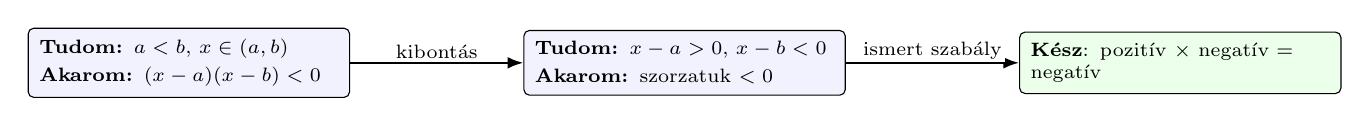
\begin{tikzpicture}[font=\small]
  \node[allapot] (A) {\textbf{Tudom:} $a<b$, $x\in(a,b)$\\[2pt] \textbf{Akarom:} $(x-a)(x-b)<0$};
  \node[allapot,right=22mm of A] (B) {\textbf{Tudom:} $x-a>0$, $x-b<0$\\[2pt] \textbf{Akarom:} szorzatuk $<0$};
  \node[cel,right=22mm of B] (C) {\textbf{Kész}: pozitív $\times$ negatív $=$ negatív};
  \draw[vnyil] (A) -- node[cimke,above] {kibontás} (B);
  \draw[vnyil] (B) -- node[cimke,above] {ismert szabály} (C);
\end{tikzpicture}
}
\end{center}

\noindent A dobozok nyelvén mindössze két mozdulat létezik:
\begin{itemize}[nosep,leftmargin=*]
  \item \textbf{Előre} (\emph{tudásból}): egy feltevésből következtetünk valamit; a felső rekesz nő.
  \item \textbf{Hátra} (\emph{célból}): a célt visszavezetjük egyszerűbb célra; az alsó rekesz változik.
\end{itemize}
A jó bizonyítás jellemzően \emph{hátulról indul} (mi kell a célhoz?), és középen találkozik
az előrefelé gyűjtött tudással. A rajzon ezt két, egymás felé haladó nyílsorral jelöljük.

\begin{center}
\resizebox{\ifdim\width>\linewidth\linewidth\else\width\fi}{!}{%
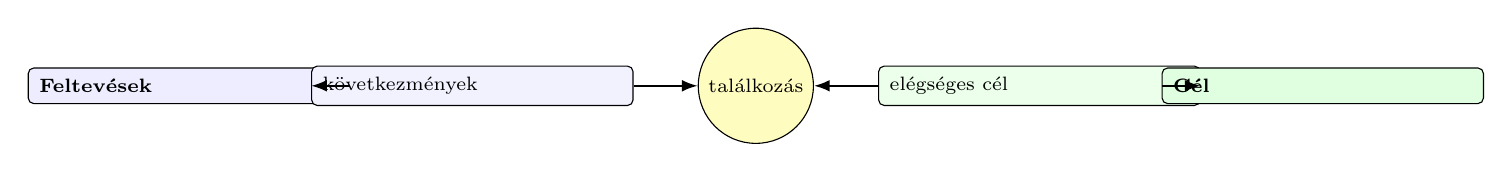
\begin{tikzpicture}[font=\small]
  \node[allapot,fill=blue!7] (T) at (0,0) {\textbf{Feltevések}};
  \node[allapot,fill=blue!5] (T2) at (3.6,0) {következmények};
  \node[draw,circle,fill=yellow!25,inner sep=3pt] (M) at (7.2,0) {\scriptsize találkozás};
  \node[cel] (C2) at (10.8,0) {elégséges cél};
  \node[cel,fill=green!12] (C) at (14.4,0) {\textbf{Cél}};
  \draw[vnyil] (T) -- (T2); \draw[vnyil] (T2) -- (M);
  \draw[vnyil] (C) -- (C2); \draw[vnyil] (C2) -- (M);
\end{tikzpicture}
}
\end{center}

\section{A hét logikai alapkocka}

Minden feladat megoldása ezekből áll össze. Mindegyikhez tartozik egy papíron írt
mondatkezdet és egy Lean-taktika --- ez a hármas (rajz / mondat / taktika) segít
átvinni a készséget egyik közegből a másikba.

\begin{center}
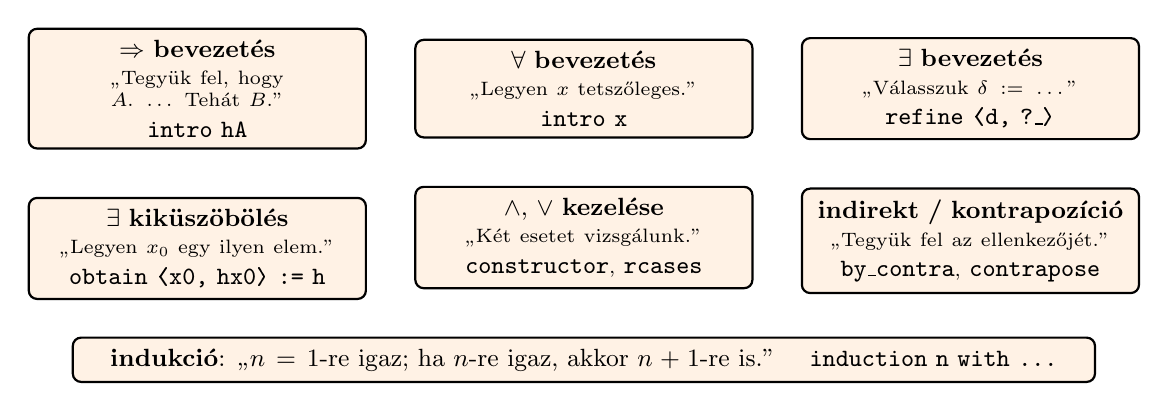
\begin{tikzpicture}[font=\small,node distance=4mm]
  \node[kocka,text width=40mm] (i1) {$\Rightarrow$ \textbf{bevezetés}\\[2pt]
     \scriptsize „Tegyük fel, hogy $A$. \dots\ Tehát $B$.”\\ \lean{intro hA}};
  \node[kocka,text width=40mm,right=6mm of i1] (i2) {$\forall$ \textbf{bevezetés}\\[2pt]
     \scriptsize „Legyen $x$ tetszőleges.”\\ \lean{intro x}};
  \node[kocka,text width=40mm,right=6mm of i2] (i3) {$\exists$ \textbf{bevezetés}\\[2pt]
     \scriptsize „Válasszuk $\delta := \dots$”\\ \lean{refine ⟨d, ?\_⟩}};
  \node[kocka,text width=40mm,below=6mm of i1] (i4) {$\exists$ \textbf{kiküszöbölés}\\[2pt]
     \scriptsize „Legyen $x_0$ egy ilyen elem.”\\ \lean{obtain ⟨x0, hx0⟩ := h}};
  \node[kocka,text width=40mm,below=6mm of i2] (i5) {$\wedge$, $\vee$ \textbf{kezelése}\\[2pt]
     \scriptsize „Két esetet vizsgálunk.”\\ \lean{constructor}, \lean{rcases}};
  \node[kocka,text width=40mm,below=6mm of i3] (i6) {\textbf{indirekt / kontrapozíció}\\[2pt]
     \scriptsize „Tegyük fel az ellenkezőjét.”\\ \lean{by\_contra}, \lean{contrapose}};
  \node[kocka,text width=127mm,below=6mm of i5] (i7) {\textbf{indukció}: „$n=1$-re igaz; ha $n$-re igaz, akkor $n+1$-re is.” \quad \lean{induction n with ...}};
\end{tikzpicture}
\end{center}

\begin{kocka}[$\forall$ és $\exists$ sorrendje]
A leggyakoribb hiba a kvantorok sorrendjének felcserélése. A rajz, ami megvéd tőle:
a \emph{játékfa} (lásd a testvérfüzetet) --- aki előbb lép, annak a választása nem
függhet a később lépő választásától. Az $\eps$--$\delta$ állításban $\delta$ függhet
$\eps$-tól, de $x$-től \emph{nem}.
\end{kocka}

\section{Nyolc összefűzési minta}

\begin{minta}[Lánc (\emph{calc})]
Egyenlőségek vagy azonos irányú egyenlőtlenségek sorozata. Rajza: vízszintes lánc,
minden nyílon az indoklás.
\end{minta}

\begin{center}
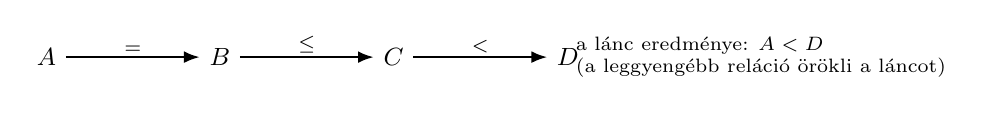
\begin{tikzpicture}[font=\small]
  \node (a) {$A$}; \node[right=17mm of a] (b) {$B$};
  \node[right=17mm of b] (c) {$C$}; \node[right=17mm of c] (d) {$D$};
  \draw[vnyil] (a) -- node[cimke,above] {$=$} (b);
  \draw[vnyil] (b) -- node[cimke,above] {$\le$} (c);
  \draw[vnyil] (c) -- node[cimke,above] {$<$} (d);
  \node[anchor=west,font=\scriptsize,align=left] at (6.6,0) {a lánc eredménye: $A<D$\\ (a leggyengébb reláció örökli a láncot)};
\end{tikzpicture}
\end{center}

\begin{minta}[Kétirányú (ekvivalencia)]
$P \iff Q$ helyett két külön nyíl. Rajza: két, ellentétes irányú félkör. Papíron:
„($\Rightarrow$)” és „($\Leftarrow$)” fejezetcímek; Leanben \lean{constructor}.
\end{minta}

\begin{minta}[Esetszétválasztás]
A fa elágazik, majd a végén az ágak \emph{ugyanabba} a célba futnak be. Rajz: fa,
alul összefutó nyilakkal. Ellenőrzés: lefedtük-e az összes esetet (ez a leggyakoribb hiányosság).
\end{minta}

\begin{center}
\resizebox{\ifdim\width>\linewidth\linewidth\else\width\fi}{!}{%
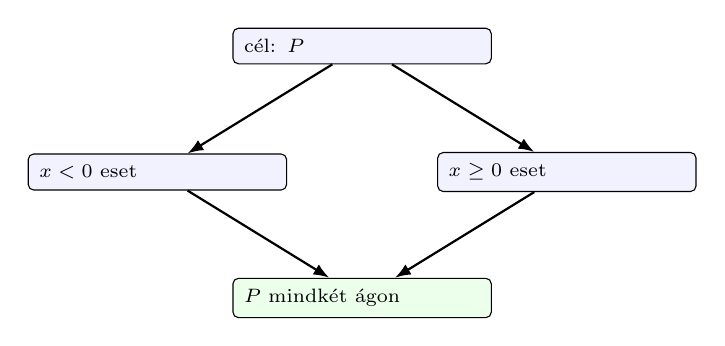
\begin{tikzpicture}[font=\small]
  \node[allapot,text width=30mm] (top) at (0,0) {cél: $P$};
  \node[allapot,text width=30mm] (l) at (-2.6,-1.6) {$x<0$ eset};
  \node[allapot,text width=30mm] (r) at (2.6,-1.6) {$x\ge0$ eset};
  \node[cel,text width=30mm] (b) at (0,-3.2) {$P$ mindkét ágon};
  \draw[vnyil] (top) -- (l); \draw[vnyil] (top) -- (r);
  \draw[vnyil] (l) -- (b); \draw[vnyil] (r) -- (b);
\end{tikzpicture}
}
\end{center}

\begin{minta}[Szendvics (rendőrelv)]
Két becslés fog közre egy mennyiséget. Rajz: két vízszintes vonal között szorult görbe.
Papíron mindig \emph{külön} bizonyítjuk az alsó és a felső becslést.
\end{minta}

\begin{minta}[Hozzáadok--kivonok (híd)]
$|A - C| \le |A-B| + |B-C|$: beszúrunk egy közbülső $B$-t. Rajz: híd két pillérrel.
Ez a mozdulat viszi a legtöbb határérték- és folytonosságbizonyítást.
\end{minta}

\begin{center}
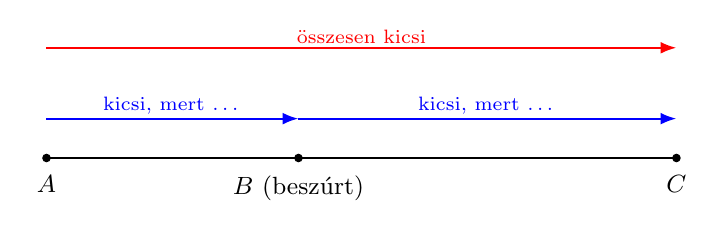
\begin{tikzpicture}[font=\small]
  \draw[seg,thick] (0,0) -- (8,0);
  \node[pont] at (0,0) {}; \node[below] at (0,-0.1) {$A$};
  \node[pont] at (3.2,0) {}; \node[below] at (3.2,-0.1) {$B$ (beszúrt)};
  \node[pont] at (8,0) {}; \node[below] at (8,-0.1) {$C$};
  \draw[vnyil,blue] (0,0.5) -- node[cimke,above] {kicsi, mert \dots} (3.2,0.5);
  \draw[vnyil,blue] (3.2,0.5) -- node[cimke,above] {kicsi, mert \dots} (8,0.5);
  \draw[vnyil,red] (0,1.4) -- node[cimke,above] {összesen kicsi} (8,1.4);
\end{tikzpicture}
\end{center}

\begin{minta}[„Elég belátni” (redukció)]
A célt kicseréljük egy erősebb, de kényelmesebb célra. Rajz: nyíl \emph{visszafelé},
a cél felől. Vigyázat: az erősebb állításnak igaznak is kell lennie.
\end{minta}

\begin{minta}[Indukció (tekercs)]
Rajz: a dominósor, de a lépés dobozában külön kiemelve, hogy \emph{mi az új tag}, amit
hozzáveszünk. A legtöbb hiba abból ered, hogy az indukciós feltevést nem használjuk fel,
vagy rossz alakban vesszük fel.
\end{minta}

\begin{minta}[Szélsőérték-mozdulat]
Egyenlőtlenséget úgy is bizonyíthatunk, hogy a különbségfüggvény szélsőértékét keressük
meg (4.8--4.11), vagy --- kompaktságon --- a \emph{legnagyobb} maximumhelyet toljuk tovább
(4.13). Rajz: a hibafüggvény grafikonja és a maximumhely mint mozgatható pont.
\end{minta}


\section{A kilenc analízis-építőkocka}

A logikai kockák fölé rakódik néhány \emph{analízis-specifikus} kocka. Mindegyikhez
tartozik egy apró ikon, amit érdemes a margóra rajzolni, amikor használjuk.

\begin{center}
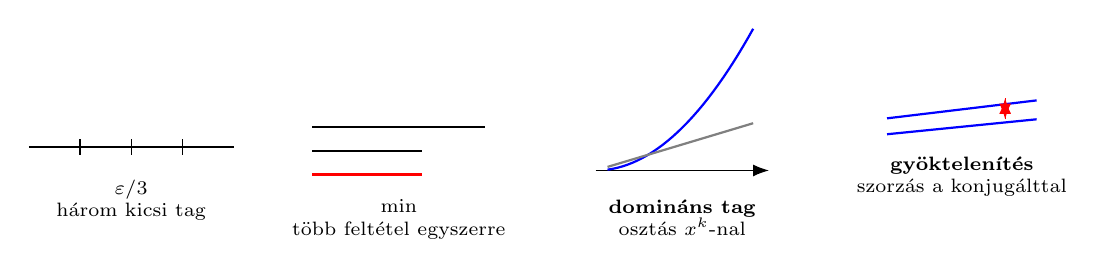
\begin{tikzpicture}[font=\scriptsize]
  % 1. eps/3
  \begin{scope}
    \draw[seg] (0,0) -- (2.6,0);
    \foreach \x in {0.65,1.3,1.95} \draw (\x,-0.1) -- (\x,0.1);
    \node[below,align=center] at (1.3,-0.3) {\textbf{$\eps/3$}\\ három kicsi tag};
  \end{scope}
  % 2. min(d1,d2)
  \begin{scope}[xshift=3.6cm]
    \draw[seg] (0,0.25) -- (2.2,0.25); \draw[seg] (0,-0.05) -- (1.4,-0.05);
    \draw[very thick,red] (0,-0.35) -- (1.4,-0.35);
    \node[below,align=center] at (1.1,-0.55) {\textbf{$\min$}\\ több feltétel egyszerre};
  \end{scope}
  % 3. dominans tag
  \begin{scope}[xshift=7.2cm]
    \draw[nyil] (0,-0.3) -- (2.2,-0.3);
    \draw[thick,blue,domain=0.15:2,samples=30] plot (\x,{-0.3+0.45*\x*\x});
    \draw[thick,gray,domain=0.15:2,samples=30] plot (\x,{-0.3+0.3*\x});
    \node[below,align=center] at (1.1,-0.55) {\textbf{domináns tag}\\ osztás $x^{k}$-nal};
  \end{scope}
  % 4. gyoktelenites
  \begin{scope}[xshift=10.8cm]
    \draw[thick,blue,domain=0.1:2,samples=30] plot (\x,{0.35+0.12*\x});
    \draw[thick,blue,domain=0.1:2,samples=30] plot (\x,{0.15+0.10*\x});
    \draw[nyil,red] (1.6,0.35) -- (1.6,0.62); \draw[nyil,red] (1.6,0.62) -- (1.6,0.35);
    \node[below,align=center] at (1.05,0.0) {\textbf{gyöktelenítés}\\ szorzás a konjugálttal};
  \end{scope}
\end{tikzpicture}

\bigskip
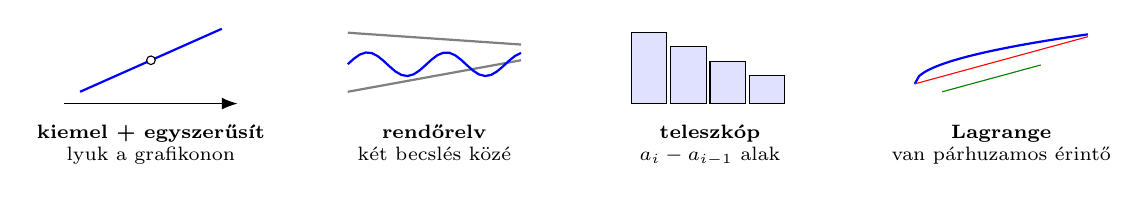
\begin{tikzpicture}[font=\scriptsize]
  % 5. kiemeles+egyszerusites
  \begin{scope}
    \draw[nyil] (0,0) -- (2.2,0);
    \draw[thick,blue] (0.2,0.15) -- (2.0,0.95);
    \node[ures] at (1.1,0.55) {};
    \node[below,align=center] at (1.1,-0.15) {\textbf{kiemel + egyszerűsít}\\ lyuk a grafikonon};
  \end{scope}
  % 6. rendorelv
  \begin{scope}[xshift=3.6cm]
    \draw[thick,gray] (0,0.9) -- (2.2,0.75); \draw[thick,gray] (0,0.15) -- (2.2,0.55);
    \draw[thick,blue,domain=0:2.2,samples=30] plot (\x,{0.5+0.15*sin(360*\x)});
    \node[below,align=center] at (1.1,-0.15) {\textbf{rendőrelv}\\ két becslés közé};
  \end{scope}
  % 7. teleszkop
  \begin{scope}[xshift=7.2cm]
    \foreach \i in {0,1,2,3} \draw[fill=blue!12] (\i*0.5,0) rectangle (\i*0.5+0.45,{0.9-0.18*\i});
    \node[below,align=center] at (1.0,-0.15) {\textbf{teleszkóp}\\ $a_i - a_{i-1}$ alak};
  \end{scope}
  % 8. Lagrange
  \begin{scope}[xshift=10.8cm]
    \draw[thick,blue,domain=0:2.2,samples=40] plot (\x,{0.25+0.6*sqrt(\x/2)});
    \draw[red] (0,0.25) -- (2.2,0.85);
    \draw[green!50!black] (0.35,0.15) -- (1.6,0.49);
    \node[below,align=center] at (1.1,-0.15) {\textbf{Lagrange}\\ van párhuzamos érintő};
  \end{scope}
\end{tikzpicture}

\bigskip

\begin{tikzpicture}[font=\scriptsize]
  \draw[seg] (0,0) -- (2.4,0); \node[pont] at (0,0) {}; \node[pont] at (2.4,0) {};
  \draw[thick,blue,domain=0:2.4,samples=40] plot (\x,{0.3+0.5*sin(75*\x)});
  \node[pont,red] at (1.2,0.78) {};
  \node[below,align=center] at (1.2,-0.15) {\textbf{kompaktság}: zárt, korlátos intervallumon a folytonos függvény felveszi a maximumát};
\end{tikzpicture}
\end{center}

\noindent Ez a kilenc kocka lefedi a 3.\ és 4.\ feladatsor szinte minden megoldását.
A feladat „megoldási terve” általában egy mondatban leírható a kockák nevével, például:
\emph{3.3 g)} $=$ gyöktelenítés $+$ domináns tag; \emph{3.7 i)} $=$ félszög-azonosság $+$
rendőrelv; \emph{4.13} $=$ kompaktság $+$ szélsőérték-mozdulat.

\section{Levezetési fák: a lépések sorrendje}

A levezetési fa alulról felfelé olvasandó: a vízszintes vonal fölött a
\emph{feltételek}, alatta a \emph{következtetés}, a vonal mellett a szabály neve.
Ez a rajz kényszerít rá, hogy minden lépéshez megnevezzük az indoklást.

\begin{center}
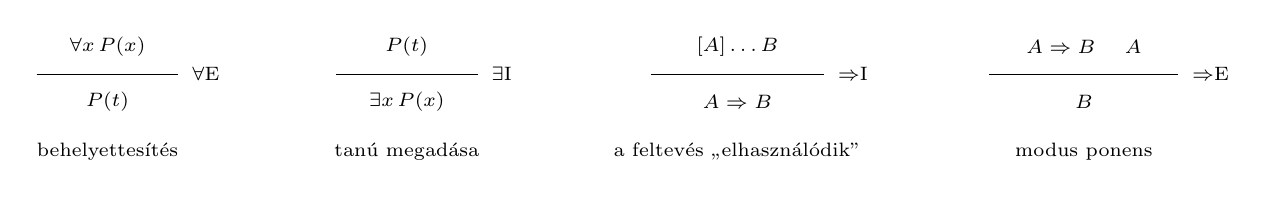
\begin{tikzpicture}[font=\scriptsize]
  \begin{scope}
    \node (a) at (0,1.2) {$\forall x\,P(x)$};
    \node (b) at (0,0.5) {$P(t)$};
    \draw (-0.9,0.85) -- (0.9,0.85); \node[anchor=west] at (0.95,0.85) {$\forall$E};
    \node[below,align=center] at (0,0.1) {behelyettesítés};
  \end{scope}
  \begin{scope}[xshift=3.8cm]
    \node (a) at (0,1.2) {$P(t)$};
    \node (b) at (0,0.5) {$\exists x\,P(x)$};
    \draw (-0.9,0.85) -- (0.9,0.85); \node[anchor=west] at (0.95,0.85) {$\exists$I};
    \node[below,align=center] at (0,0.1) {tanú megadása};
  \end{scope}
  \begin{scope}[xshift=8.0cm]
    \node (a) at (0,1.2) {$[A] \dots B$};
    \node (b) at (0,0.5) {$A \Rightarrow B$};
    \draw (-1.1,0.85) -- (1.1,0.85); \node[anchor=west] at (1.15,0.85) {$\Rightarrow$I};
    \node[below,align=center] at (0,0.1) {a feltevés „elhasználódik”};
  \end{scope}
  \begin{scope}[xshift=12.4cm]
    \node (a) at (0,1.2) {$A\Rightarrow B$ \quad $A$};
    \node (b) at (0,0.5) {$B$};
    \draw (-1.2,0.85) -- (1.2,0.85); \node[anchor=west] at (1.25,0.85) {$\Rightarrow$E};
    \node[below,align=center] at (0,0.1) {modus ponens};
  \end{scope}
\end{tikzpicture}
\end{center}

\noindent Példa teljes fára (1.13, általánosított háromszög-egyenlőtlenség, indukciós lépés):

\begin{center}
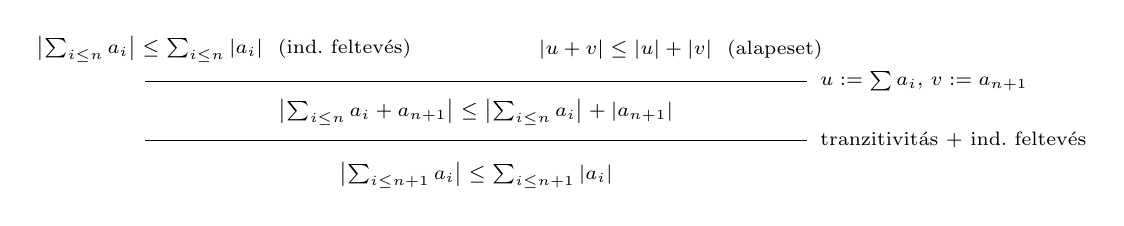
\begin{tikzpicture}[font=\scriptsize]
  \node (h1) at (-3.2,2.2) {$\bigl|\sum_{i\le n} a_i\bigr| \le \sum_{i\le n} |a_i|$ \ (ind.\ feltevés)};
  \node (h2) at (2.6,2.2) {$|u+v| \le |u|+|v|$ \ (alapeset)};
  \node (c1) at (0,1.4) {$\bigl|\sum_{i\le n} a_i + a_{n+1}\bigr| \le \bigl|\sum_{i\le n} a_i\bigr| + |a_{n+1}|$};
  \draw (-4.2,1.8) -- (4.2,1.8); \node[anchor=west] at (4.25,1.8) {$u:=\sum a_i$, $v:=a_{n+1}$};
  \node (c2) at (0,0.6) {$\bigl|\sum_{i\le n+1} a_i\bigr| \le \sum_{i\le n+1} |a_i|$};
  \draw (-4.2,1.05) -- (4.2,1.05); \node[anchor=west] at (4.25,1.05) {tranzitivitás $+$ ind.\ feltevés};
\end{tikzpicture}
\end{center}

\section{Az indukció három rajza}

\begin{center}
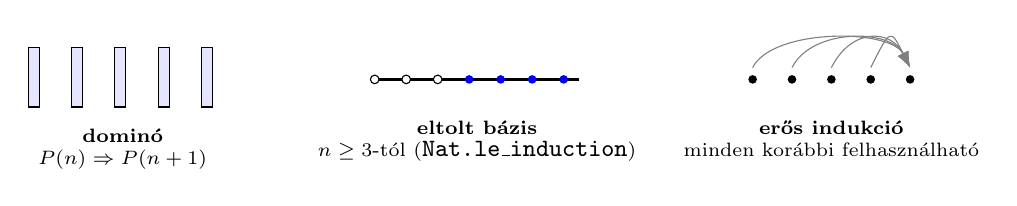
\begin{tikzpicture}[font=\scriptsize]
  % domino
  \begin{scope}
    \foreach \i in {0,...,4} \draw[fill=blue!10] (\i*0.55,0) rectangle (\i*0.55+0.14,0.75);
    \node[below,align=center] at (1.2,-0.15) {\textbf{dominó}\\ $P(n)\Rightarrow P(n+1)$};
  \end{scope}
  % eltolt bazis
  \begin{scope}[xshift=4.4cm]
    \draw[seg] (0,0.35) -- (2.6,0.35);
    \foreach \i in {0,1,2} \node[ures] at (\i*0.4,0.35) {};
    \foreach \i in {3,...,6} \node[pont,blue] at (\i*0.4,0.35) {};
    \node[below,align=center] at (1.3,-0.05) {\textbf{eltolt bázis}\\ $n\ge3$-tól (\lean{Nat.le\_induction})};
  \end{scope}
  % eros indukcio
  \begin{scope}[xshift=9.2cm]
    \foreach \i in {0,...,4} \node[pont] at (\i*0.5,0.35) {};
    \foreach \i in {0,...,3} \draw[nyil,gray] (\i*0.5,0.5) .. controls +(0.25,0.5) and +(-0.25,0.5) .. (2.0,0.5);
    \node[below,align=center] at (1.0,-0.05) {\textbf{erős indukció}\\ minden korábbi felhasználható};
  \end{scope}
\end{tikzpicture}
\end{center}

\noindent A második rajz azért fontos, mert több feladat (1.15 c), 1.18, 3.16) csak
egy bizonyos indextől igaz; ilyenkor a bázis nem $n=0$, hanem az első jó index.


\section{Tizenkét bizonyítás lépésről lépésre}

Az alábbi rajzcsíkok mindegyike egy-egy gyakorlat teljes vázát adja. A csík dobozai az
állapotokat, a nyilak a lépéseket mutatják; a csík alatt a hozzá tartozó \emph{kép}
és a Lean-tétel neve áll.

\subsection{1.11 --- fordított háromszög-egyenlőtlenség}

\begin{center}
\resizebox{\ifdim\width>\linewidth\linewidth\else\width\fi}{!}{%
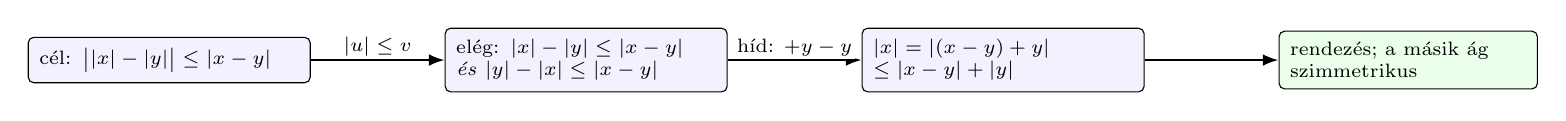
\begin{tikzpicture}[font=\small]
  \node[allapot,text width=33mm] (a) {cél: $\bigl||x|-|y|\bigr|\le|x-y|$};
  \node[allapot,text width=33mm,right=17mm of a] (b) {elég: $|x|-|y|\le|x-y|$\\ \emph{és} $|y|-|x|\le|x-y|$};
  \node[allapot,text width=33mm,right=17mm of b] (c) {$|x| = |(x-y)+y|$\\ $\le |x-y|+|y|$};
  \node[cel,text width=30mm,right=17mm of c] (d) {rendezés; a másik ág szimmetrikus};
  \draw[vnyil] (a) -- node[cimke,above] {$|u|\le v$} (b);
  \draw[vnyil] (b) -- node[cimke,above] {híd: $+y-y$} (c);
  \draw[vnyil] (c) -- (d);
\end{tikzpicture}
}
\end{center}

\noindent \emph{Kép}: a számegyenesen $x$, $0$, $y$; a „kerülő nem rövidebb”.
\emph{Lean}: \lean{Szakasz1.gyak\_1\_11}.

\subsection{1.12 a) --- abszolút értékes egyenlőtlenség}

\begin{center}
\resizebox{\ifdim\width>\linewidth\linewidth\else\width\fi}{!}{%
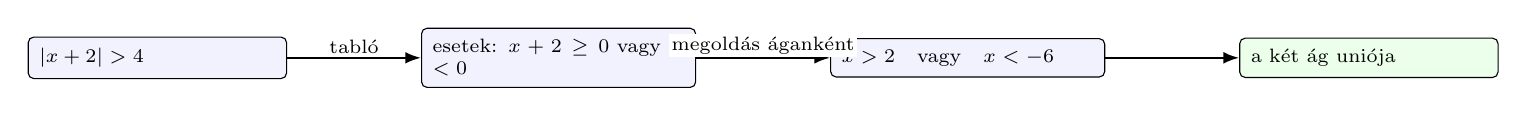
\begin{tikzpicture}[font=\small]
  \node[allapot,text width=30mm] (a) {$|x+2|>4$};
  \node[allapot,text width=32mm,right=17mm of a] (b) {esetek: $x+2\ge0$ vagy $<0$};
  \node[allapot,text width=32mm,right=17mm of b] (c) {$x>2$ \ \ vagy \ \ $x<-6$};
  \node[cel,text width=30mm,right=17mm of c] (d) {a két ág uniója};
  \draw[vnyil] (a) -- node[cimke,above] {tabló} (b);
  \draw[vnyil] (b) -- node[cimke,above] {megoldás áganként} (c);
  \draw[vnyil] (c) -- (d);
\end{tikzpicture}
}
\end{center}

\noindent \emph{Kép}: számegyenes két sávval. \emph{Lean}: \lean{Szakasz1.gyak\_1\_12\_a}.
Figyeljünk arra, hogy a végeredményt \emph{halmazként} írjuk le --- az „és/vagy”
felcserélése itt a tipikus hiba.

\subsection{1.14 a) --- Gauss-összeg indukcióval}

\begin{center}
\resizebox{\ifdim\width>\linewidth\linewidth\else\width\fi}{!}{%
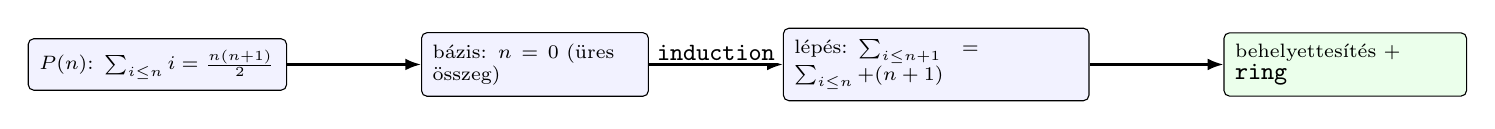
\begin{tikzpicture}[font=\small]
  \node[allapot,text width=30mm] (a) {$P(n)$: $\sum_{i\le n} i = \frac{n(n+1)}{2}$};
  \node[allapot,text width=26mm,right=17mm of a] (b) {bázis: $n=0$ (üres összeg)};
  \node[allapot,text width=36mm,right=17mm of b] (c) {lépés: $\sum_{i\le n+1} = \sum_{i\le n} + (n+1)$};
  \node[cel,text width=28mm,right=17mm of c] (d) {behelyettesítés + \lean{ring}};
  \draw[vnyil] (a) -- (b); \draw[vnyil] (b) -- node[cimke,above] {\lean{induction}} (c); \draw[vnyil] (c) -- (d);
\end{tikzpicture}
}
\end{center}

\noindent \emph{Kép}: két lépcső egy téglalapban. \emph{Lean}: \lean{Szakasz1.gyak\_1\_14\_a},
illetve indukció nélkül \lean{Rajzok.gauss\_teglalap}.

\subsection{1.15 c) --- teleszkópos becslés}

\begin{center}
\resizebox{\ifdim\width>\linewidth\linewidth\else\width\fi}{!}{%
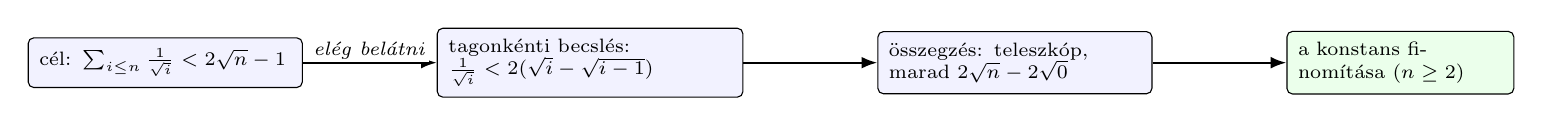
\begin{tikzpicture}[font=\small]
  \node[allapot,text width=32mm] (a) {cél: $\sum_{i\le n} \frac{1}{\sqrt i} < 2\sqrt n - 1$};
  \node[allapot,text width=36mm,right=17mm of a] (b) {tagonkénti becslés:\\ $\frac{1}{\sqrt i} < 2(\sqrt i - \sqrt{i-1})$};
  \node[allapot,text width=32mm,right=17mm of b] (c) {összegzés: teleszkóp,\\ marad $2\sqrt n - 2\sqrt 0$};
  \node[cel,text width=26mm,right=17mm of c] (d) {a konstans finomítása ($n\ge2$)};
  \draw[vnyil] (a) -- node[cimke,above] {\emph{elég belátni}} (b);
  \draw[vnyil] (b) -- (c); \draw[vnyil] (c) -- (d);
\end{tikzpicture}
}
\end{center}

\noindent \emph{Kép}: téglalapok az $1/\sqrt x$ görbe alatt. \emph{Lean}:
\lean{Szakasz1.gyak\_1\_15\_c\_also}, \lean{gyak\_1\_15\_c\_felso}. A felső becslés
$n=1$-re \emph{nem} igaz (ott egyenlőség áll) --- ezt a rajz is mutatja, ha a legelső
téglalapot külön megnézzük.

\subsection{1.18 --- rekurzív sorozat, pókháló}

\begin{center}
\resizebox{\ifdim\width>\linewidth\linewidth\else\width\fi}{!}{%
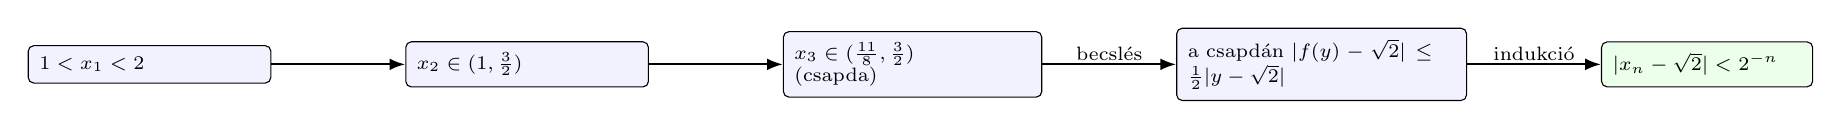
\begin{tikzpicture}[font=\small]
  \node[allapot,text width=28mm] (a) {$1<x_1<2$};
  \node[allapot,text width=28mm,right=17mm of a] (b) {$x_2 \in (1,\tfrac32)$};
  \node[allapot,text width=30mm,right=17mm of b] (c) {$x_3 \in (\tfrac{11}{8},\tfrac32)$ \\ (csapda)};
  \node[allapot,text width=34mm,right=17mm of c] (d) {a csapdán $|f(y)-\sqrt2| \le \tfrac12|y-\sqrt2|$};
  \node[cel,text width=24mm,right=17mm of d] (e) {$|x_n-\sqrt2|<2^{-n}$};
  \draw[vnyil] (a) -- (b); \draw[vnyil] (b) -- (c);
  \draw[vnyil] (c) -- node[cimke,above] {becslés} (d);
  \draw[vnyil] (d) -- node[cimke,above] {indukció} (e);
\end{tikzpicture}
}
\end{center}

\noindent \emph{Kép}: pókháló-diagram. \emph{Lean}: \lean{Rajzok.gyak\_1\_18},
általánosan \lean{Rajzok.pokhalo\_zsugorodas}. A kulcslépés a \emph{csapdaintervallum}
megtalálása: a rajzon látszik, hogy két lépés után a sorozat egy szűk sávba kerül,
és ott a meredekség már $1/2$ alatt van.

\subsection{2.18 --- injektív függvények kompozíciója}

\begin{center}
\resizebox{\ifdim\width>\linewidth\linewidth\else\width\fi}{!}{%
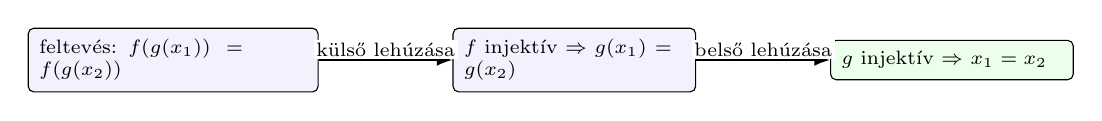
\begin{tikzpicture}[font=\small]
  \node[allapot,text width=34mm] (a) {feltevés: $f(g(x_1))=f(g(x_2))$};
  \node[allapot,text width=28mm,right=17mm of a] (b) {$f$ injektív $\Rightarrow$ $g(x_1)=g(x_2)$};
  \node[cel,text width=28mm,right=17mm of b] (c) {$g$ injektív $\Rightarrow$ $x_1=x_2$};
  \draw[vnyil] (a) -- node[cimke,above] {külső lehúzása} (b);
  \draw[vnyil] (b) -- node[cimke,above] {belső lehúzása} (c);
\end{tikzpicture}
}
\end{center}

\noindent \emph{Kép}: nyíldiagram $X\to Y\to Z$; a mono-tulajdonság „balról
egyszerűsítés”. \emph{Lean}: \lean{Szakasz2.gyak\_2\_18}, kategóriaelméleti alakban
\lean{Kategoria.mono\_comp\_mono}.

\subsection{2.19 --- $n$-edfokú polinomnak legfeljebb $n$ gyöke van}

\begin{center}
\resizebox{\ifdim\width>\linewidth\linewidth\else\width\fi}{!}{%
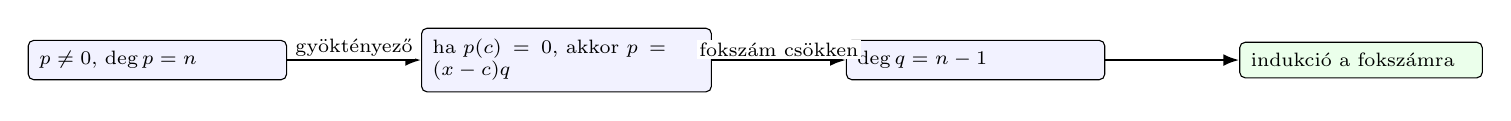
\begin{tikzpicture}[font=\small]
  \node[allapot,text width=30mm] (a) {$p \ne 0$, $\deg p = n$};
  \node[allapot,text width=34mm,right=17mm of a] (b) {ha $p(c)=0$, akkor $p=(x-c)q$};
  \node[allapot,text width=30mm,right=17mm of b] (c) {$\deg q = n-1$};
  \node[cel,text width=28mm,right=17mm of c] (d) {indukció a fokszámra};
  \draw[vnyil] (a) -- node[cimke,above] {gyöktényező} (b);
  \draw[vnyil] (b) -- node[cimke,above] {fokszám csökken} (c);
  \draw[vnyil] (c) -- (d);
\end{tikzpicture}
}
\end{center}

\noindent \emph{Kép}: a grafikon minden gyöknél „levág” egy tényezőt; lefelé lépcsőző fa.
\emph{Lean}: \lean{Szakasz2.gyak\_2\_19}.

\subsection{3.1 a) --- $\eps$--$\delta$ visszafejtés}

Az $\eps$--$\delta$ bizonyítás \emph{piszkozata} mindig hátulról készül: a célból
számoljuk ki, mekkora $\delta$ kell. A tisztázatban ez megfordul.

\begin{center}
\resizebox{\ifdim\width>\linewidth\linewidth\else\width\fi}{!}{%
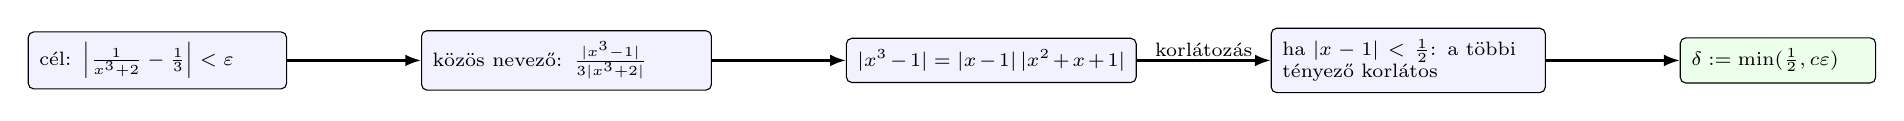
\begin{tikzpicture}[font=\small]
  \node[allapot,text width=30mm] (a) {cél: $\left|\frac{1}{x^3+2}-\frac13\right|<\eps$};
  \node[allapot,text width=34mm,right=17mm of a] (b) {közös nevező: $\frac{|x^3-1|}{3|x^3+2|}$};
  \node[allapot,text width=34mm,right=17mm of b] (c) {$|x^3-1| = |x-1|\,|x^2+x+1|$};
  \node[allapot,text width=32mm,right=17mm of c] (d) {ha $|x-1|<\tfrac12$: a többi tényező korlátos};
  \node[cel,text width=22mm,right=17mm of d] (e) {$\delta := \min(\tfrac12, c\eps)$};
  \draw[vnyil] (a) -- (b); \draw[vnyil] (b) -- (c);
  \draw[vnyil] (c) -- node[cimke,above] {korlátozás} (d); \draw[vnyil] (d) -- (e);
\end{tikzpicture}
}
\end{center}

\noindent \emph{Kép}: $\eps$--$\delta$ doboz. \emph{Lean}:
\lean{Szakasz3.gyak\_3\_1\_a\_epsdelta}. A „$\min$” a rajzon két korlátozás metszete:
egy \emph{előzetes} szűkítés (hogy a zavaró tényezőket becsülni tudjuk) és a
\emph{tényleges} $\eps$-tól függő szűkítés.

\subsection{3.4 --- $0/0$ típus, gyöktényező kiemelése}

\begin{center}
\resizebox{\ifdim\width>\linewidth\linewidth\else\width\fi}{!}{%
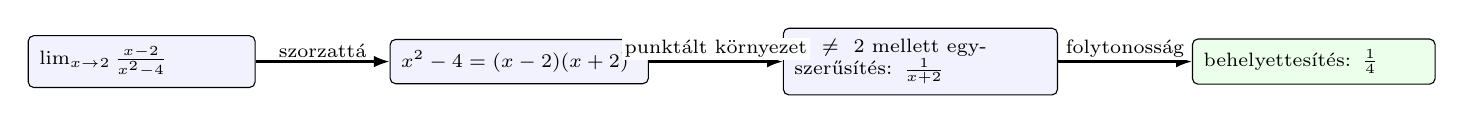
\begin{tikzpicture}[font=\small]
  \node[allapot,text width=26mm] (a) {$\lim_{x\to2}\frac{x-2}{x^2-4}$};
  \node[allapot,text width=30mm,right=17mm of a] (b) {$x^2-4=(x-2)(x+2)$};
  \node[allapot,text width=32mm,right=17mm of b] (c) {$x\ne2$ mellett egyszerűsítés: $\frac{1}{x+2}$};
  \node[cel,text width=28mm,right=17mm of c] (d) {behelyettesítés: $\tfrac14$};
  \draw[vnyil] (a) -- node[cimke,above] {szorzattá} (b);
  \draw[vnyil] (b) -- node[cimke,above] {punktált környezet} (c);
  \draw[vnyil] (c) -- node[cimke,above] {folytonosság} (d);
\end{tikzpicture}
}
\end{center}

\noindent \emph{Kép}: lyukas grafikon. \emph{Lean}: \lean{Szakasz3.gyak\_3\_4\_a}.
A második nyíl fogalmi lényege: a határértéknél a pont \emph{maga} nem számít, ezért
szabad $x\ne2$ mellett egyszerűsíteni.

\subsection{3.7 --- $\sin x / x$ rendőrelvvel}

\begin{center}
\resizebox{\ifdim\width>\linewidth\linewidth\else\width\fi}{!}{%
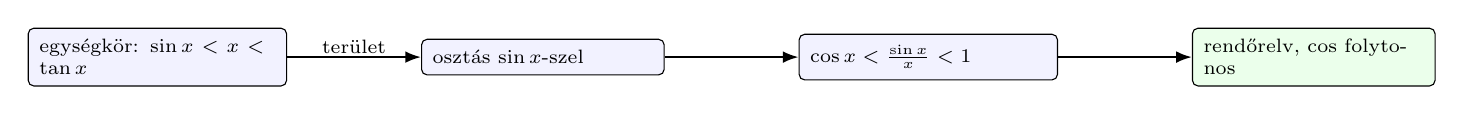
\begin{tikzpicture}[font=\small]
  \node[allapot,text width=30mm] (a) {egységkör: $\sin x < x < \tan x$};
  \node[allapot,text width=28mm,right=17mm of a] (b) {osztás $\sin x$-szel};
  \node[allapot,text width=30mm,right=17mm of b] (c) {$\cos x < \frac{\sin x}{x} < 1$};
  \node[cel,text width=28mm,right=17mm of c] (d) {rendőrelv, $\cos$ folytonos};
  \draw[vnyil] (a) -- node[cimke,above] {terület} (b);
  \draw[vnyil] (b) -- (c); \draw[vnyil] (c) -- (d);
\end{tikzpicture}
}
\end{center}

\noindent \emph{Kép}: körcikk-szendvics. \emph{Lean}: \lean{Rajzok.egysegkor\_szendvics},
\lean{Rajzok.rendorelv\_sav}, \lean{Szakasz3.gyak\_3\_7\_alap}.

\subsection{3.14 --- monoton, korlátos $\Rightarrow$ létezik a bal oldali határérték}

\begin{center}
\resizebox{\ifdim\width>\linewidth\linewidth\else\width\fi}{!}{%
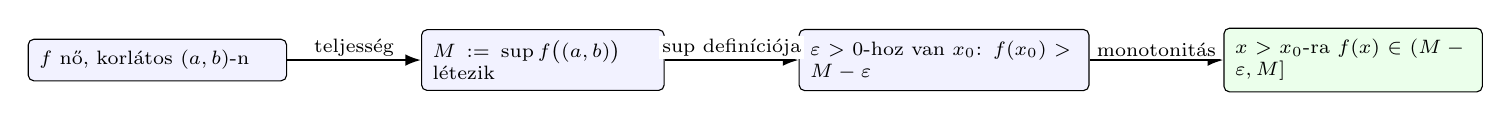
\begin{tikzpicture}[font=\small]
  \node[allapot,text width=30mm] (a) {$f$ nő, korlátos $(a,b)$-n};
  \node[allapot,text width=28mm,right=17mm of a] (b) {$M := \sup f\bigl((a,b)\bigr)$ létezik};
  \node[allapot,text width=34mm,right=17mm of b] (c) {$\eps>0$-hoz van $x_0$: $f(x_0)>M-\eps$};
  \node[cel,text width=30mm,right=17mm of c] (d) {$x>x_0$-ra $f(x)\in(M-\eps,M]$};
  \draw[vnyil] (a) -- node[cimke,above] {teljesség} (b);
  \draw[vnyil] (b) -- node[cimke,above] {$\sup$ definíciója} (c);
  \draw[vnyil] (c) -- node[cimke,above] {monotonitás} (d);
\end{tikzpicture}
}
\end{center}

\noindent \emph{Kép}: plafon-rajz. \emph{Lean}: \lean{Szakasz3.gyak\_3\_14}.
Ez a csík mutatja a legszebben a „teljesség $\to$ létezés” mintát: először
\emph{létrehozzuk} a határérték jelöltjét, és csak utána bizonyítjuk róla, hogy jó.

\subsection{4.13 --- középponti konvexitás $+$ folytonosság $\Rightarrow$ konvexitás}

\begin{center}
\resizebox{\ifdim\width>\linewidth\linewidth\else\width\fi}{!}{%
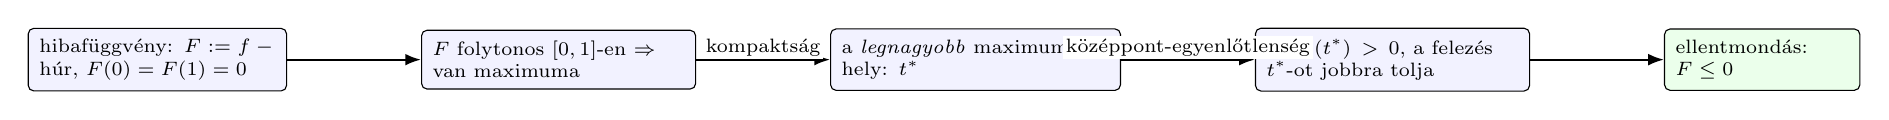
\begin{tikzpicture}[font=\small]
  \node[allapot,text width=30mm] (a) {hibafüggvény: $F := f - \text{húr}$, $F(0)=F(1)=0$};
  \node[allapot,text width=32mm,right=17mm of a] (b) {$F$ folytonos $[0,1]$-en $\Rightarrow$ van maximuma};
  \node[allapot,text width=34mm,right=17mm of b] (c) {a \emph{legnagyobb} maximumhely: $t^*$};
  \node[allapot,text width=32mm,right=17mm of c] (d) {ha $F(t^*)>0$, a felezés $t^*$-ot jobbra tolja};
  \node[cel,text width=22mm,right=17mm of d] (e) {ellentmondás: $F\le0$};
  \draw[vnyil] (a) -- (b); \draw[vnyil] (b) -- node[cimke,above] {kompaktság} (c);
  \draw[vnyil] (c) -- node[cimke,above] {középpont-egyenlőtlenség} (d);
  \draw[vnyil] (d) -- (e);
\end{tikzpicture}
}
\end{center}

\noindent \emph{Kép}: a húr alatti hibafüggvény és a jobbra tolható maximumhely.
\emph{Lean}: \lean{Szakasz4.kozeppontos\_nonpos\_of\_endpoints} és
\lean{Szakasz4.gyak\_4\_13}.

\section{Ugyanaz a bizonyítás háromféle rajzban}

Érdemes egyszer végigcsinálni, hogy ugyanazt a gondolatmenetet háromféleképp is
lerajzoljuk. Példa: \emph{2.18}, injektív függvények kompozíciója.

\begin{center}
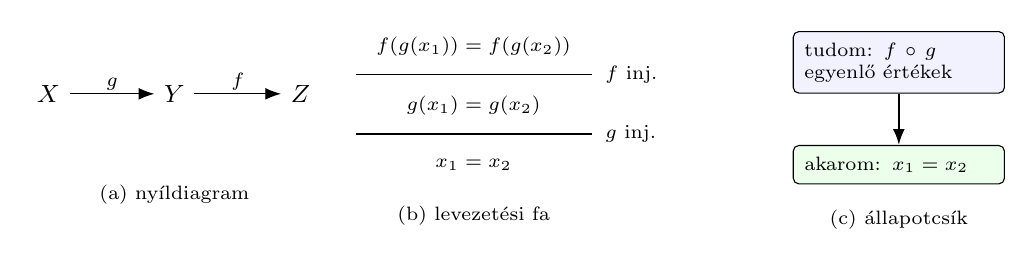
\begin{tikzpicture}[font=\small]
  % 1. nyíldiagram
  \begin{scope}
    \node (X) at (0,0) {$X$}; \node (Y) at (1.6,0) {$Y$}; \node (Z) at (3.2,0) {$Z$};
    \draw[nyil] (X) -- node[cimke,above] {$g$} (Y);
    \draw[nyil] (Y) -- node[cimke,above] {$f$} (Z);
    \node[below=8mm of Y,font=\scriptsize,align=center] {(a) nyíldiagram};
  \end{scope}
  % 2. levezetesi fa
  \begin{scope}[xshift=5.4cm,yshift=0.6cm]
    \node (top) at (0,0) {\scriptsize $f(g(x_1))=f(g(x_2))$};
    \node (mid) at (0,-0.75) {\scriptsize $g(x_1)=g(x_2)$};
    \node (bot) at (0,-1.5) {\scriptsize $x_1=x_2$};
    \draw (-1.5,-0.36) -- (1.5,-0.36); \node[anchor=west,font=\scriptsize] at (1.55,-0.36) {$f$ inj.};
    \draw (-1.5,-1.11) -- (1.5,-1.11); \node[anchor=west,font=\scriptsize] at (1.55,-1.11) {$g$ inj.};
    \node[below=2mm of bot,font=\scriptsize,align=center] {(b) levezetési fa};
  \end{scope}
  % 3. allapotcsik
  \begin{scope}[xshift=10.8cm]
    \node[allapot,text width=24mm] (s1) at (0,0.4) {tudom: $f\circ g$ egyenlő értékek};
    \node[cel,text width=24mm] (s2) at (0,-0.9) {akarom: $x_1=x_2$};
    \draw[vnyil] (s1) -- (s2);
    \node[below=2mm of s2,font=\scriptsize,align=center] {(c) állapotcsík};
  \end{scope}
\end{tikzpicture}
\end{center}

\noindent A három nézet ugyanaz: (a) mutatja a \emph{struktúrát}, (b) a
\emph{sorrendet}, (c) pedig azt, hogy éppen \emph{hol tartunk}. Vizsgán az (c) nézet a
leghasznosabb, mert megakadályozza, hogy elveszítsük a fonalat; a jegyzetben az (a);
a Lean-kódban gyakorlatilag a (b) jelenik meg.

\section{Papír $\leftrightarrow$ Lean szótár}

\begingroup
\small
\begin{longtable}{@{}p{4.4cm}p{5.4cm}p{4.6cm}@{}}
\toprule
\textbf{Mozdulat} & \textbf{Papíron} & \textbf{Leanben} \\
\midrule
\endfirsthead
\toprule
\textbf{Mozdulat} & \textbf{Papíron} & \textbf{Leanben} \\
\midrule
\endhead
\bottomrule
\endfoot
feltevés felvétele & „Tegyük fel, hogy $A$.” & \lean{intro hA} \\
tetszőleges elem & „Legyen $x$ tetszőleges.” & \lean{intro x} \\
tanú megadása & „Válasszuk $\delta:=\min(1,\eps/3)$.” & \lean{refine ⟨\_, ?\_⟩} \\
egzisztencia kibontása & „Legyen $x_0$ egy ilyen.” & \lean{obtain ⟨x0, hx0⟩ := h} \\
eset szétválasztás & „Két eset lehetséges.” & \lean{rcases}, \lean{by\_cases} \\
és-kettévágás & „Két állítást bizonyítunk.” & \lean{constructor} \\
lánc & „$A = B \le C < D$” & \lean{calc} \\
átrendezés, azonosság & „rendezés után” & \lean{ring}, \lean{field\_simp} \\
lineáris becslés & „innen már következik” & \lean{linarith}, \lean{nlinarith} \\
indirekt & „Tegyük fel az ellenkezőjét.” & \lean{by\_contra h} \\
kontrapozíció & „Elég a megfordítottját.” & \lean{contrapose!} \\
indukció & „$n$-re: bázis és lépés” & \lean{induction n with} \\
indukció $k$-tól & „$n\ge3$-tól indul” & \lean{Nat.le\_induction} \\
kvantorok tagadása & „nem minden $\dots$, tehát van $\dots$” & \lean{push\_neg} \\
korábbi tétel behívása & „a 3.7 szerint” & \lean{exact}, \lean{apply} \\
rendőrelv & „két becslés közé szorítjuk” & \lean{squeeze\_zero}, illetve a szűrős alakú rendőrelv-lemma \\
kompaktsági érvelés & „a maximum felvétetik” & \lean{IsCompact.exists\_isMaxOn} \\
\end{longtable}
\endgroup

\section{Hibakereső: mikor rossz a kocka?}

\begin{enumerate}[nosep,leftmargin=*]
  \item \textbf{Körkörösség}: a bizonyítandót használjuk fel. Rajzban azonnal látszik:
        a nyíl visszamutat egy korábbi dobozra.
  \item \textbf{Kvantorcsere}: $\delta$ függ $x$-től. A játékfa megvéd tőle.
  \item \textbf{Osztás ismeretlen előjelűvel / nullával}: egyenlőtlenségnél irányt vált,
        egyenletnél gyököt veszít. Ellenszer: előjelvonal vagy tabló.
  \item \textbf{Hiányzó eset}: a fa egyik ága lemarad (pl.\ $x<0$ a gyökös feladatokban).
  \item \textbf{Perempont}: nyitott/zárt intervallum keverése (1.4 b, 4.9 végpontjai).
  \item \textbf{„A rajzról látszik”}: a kép sejtést ad, nem bizonyítást --- a
        3.15 és a 4.13 feladat pont arról szól, hogy a szemléletes állítást
        \emph{miért} kell külön igazolni.
  \item \textbf{Rossz irányú L'Hospital}: nem $0/0$ vagy $\infty/\infty$ alak, vagy a
        derivált hányadosának nincs határértéke.
\end{enumerate}

\section{Sablonok másoláshoz}

Ezt a két üres sablont érdemes a füzet elejére lerajzolni, és minden feladatnál kitölteni.

\begin{center}
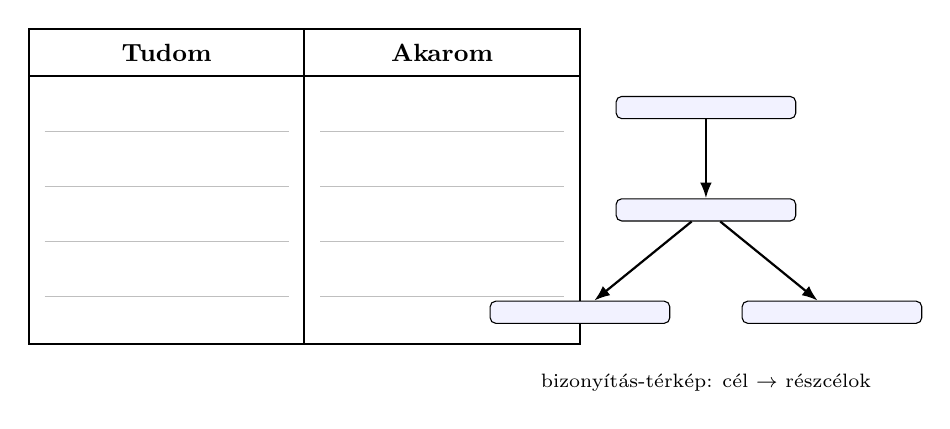
\begin{tikzpicture}[font=\small]
  % ket oszlop sablon
  \draw[thick] (0,0) rectangle (7,4);
  \draw[thick] (3.5,0) -- (3.5,4);
  \draw[thick] (0,3.4) -- (7,3.4);
  \node at (1.75,3.7) {\textbf{Tudom}};
  \node at (5.25,3.7) {\textbf{Akarom}};
  \foreach \y in {0.6,1.3,2.0,2.7} {
    \draw[gray!50] (0.2,\y) -- (3.3,\y);
    \draw[gray!50] (3.7,\y) -- (6.8,\y);
  }
  % terkep sablon
  \begin{scope}[xshift=8.6cm,yshift=0.4cm]
    \node[allapot,text width=20mm] (a) at (0,2.6) {};
    \node[allapot,text width=20mm] (b) at (0,1.3) {};
    \node[allapot,text width=20mm] (c1) at (-1.6,0) {};
    \node[allapot,text width=20mm] (c2) at (1.6,0) {};
    \draw[vnyil] (a) -- (b);
    \draw[vnyil] (b) -- (c1); \draw[vnyil] (b) -- (c2);
    \node[font=\scriptsize] at (0,-0.9) {bizonyítás-térkép: cél $\to$ részcélok};
  \end{scope}
\end{tikzpicture}
\end{center}

\bigskip
\noindent\textbf{Kapcsolódó anyagok.}
\begin{itemize}[nosep,leftmargin=*]
  \item \lean{kalkulus\_rajzos\_gondolkodas.pdf} --- rajzcsaládok feladatonként;
  \item \lean{kalkulus\_kategoriaelmelet.pdf} --- tematika-megfeleltetés és
        kategóriaelméleti olvasat;
  \item \lean{RequestProject/} --- a formalizált, \lean{sorry} nélküli Lean-bizonyítások.
\end{itemize}

\end{document}
